\documentclass{article}
\usepackage{iclr2027_conference,times}
\usepackage[utf8]{inputenc}
\usepackage[T1]{fontenc}
\usepackage{amsmath,amssymb,booktabs,graphicx,xspace}
\usepackage[hidelinks]{hyperref}
\usepackage{url}
\hypersetup{pdftitle={Relevance Labels and Source Identity Can Change Scientific Retrieval Conclusions: A CER-Bench Audit},pdfauthor={Anonymous Authors}}
\newcommand{\cer}{\textsc{CER-Bench}\xspace}
\newcommand{\Rtwenty}{\mathrm{R}@20}
\newcommand{\ind}{\mathbf{1}}
\title{Relevance Labels and Source Identity Can Change Scientific Retrieval Conclusions: A CER-Bench Audit}
\author{Anonymous Authors}
\begin{document}
\maketitle

\begin{abstract}
Scientific retrieval evaluation depends on both which documents are labeled relevant and whether their identifiers refer to the intended sources. We audit these dependencies in \cer, a historical collection of 304 synthetic biomedical tasks. An authoritative re-fetch of all 4,936 corpus PubMed records identifies a parser error that could assign cited-paper identifiers to the current article: 247 PMC identifiers change, and 226 changed historical PMC identifiers occur in reference lists. Separately, recomputation on fixed historical rankings finds nine pairwise system-order reversals between seed and expanded relevance labels. A controlled experiment with 1,000 paired, nested disclosures of existing judgments changes the mean token-recall leader between the tested fractions 0.2 and 0.3; paired empirical intervals overlap zero at both points. These are historical identifier-level diagnostics, not validated biomedical rankings. We also construct a source-identity-checked retrieval dataset with 4,936 documents and 10,313 chunks, restoring conservative own-article body text for 525 documents, and verify local BM25 execution without relevance scoring. No human relevance validation, new model experiments, or corrected-corpus leaderboard are available. The contribution is a joint provenance and evaluation audit, with explicit boundaries between arithmetic reproducibility, source ownership, and scientific validity.
\end{abstract}

\section{Introduction}
Scientific search often asks for an evidence set rather than an isolated topically similar paper. A comparison requires both sides; a multi-paper argument requires a valid chain; and a constrained question may require one study satisfying several conditions jointly. Evaluating these requests requires more than a ranking function. It requires trustworthy source identities, an appropriate relevance relation, and a metric whose success condition matches the scientific question.

Incomplete judgments and assessor variation are established problems in information retrieval (IR) \citep{buckley2004incomplete,voorhees2000judgments}. We do not claim that ranking sensitivity to labels is new. Instead, we examine what remains defensible when label sensitivity coexists with a source-identity failure in a scientific retrieval collection. A score can be exactly reproducible while its biomedical interpretation is unsupported: matching two identifier strings does not establish that either string was attached to the intended article text.

\cer originally paired synthetic questions with a biomedical corpus and saved outputs from lexical, dense, sparse, fusion, reranking, and agentic retrieval configurations. Its construction made two dependencies particularly important. Generating source papers were retained as positive seed labels, whereas additional candidates received automated judgments. Separately, source identifiers linked PubMed metadata to locally stored article XML. This audit finds problems at both boundaries. The labels change the ordering of fixed saved systems, and an overly broad XML traversal could substitute identifiers from references for the current article's identifiers.

Our question is therefore not which retriever wins a repaired benchmark. It is \emph{which conclusions survive an explicit separation of historical arithmetic, authoritative source identity, and validated relevance?} We address this through three empirical components and a bounded software contribution. First, an all-record PubMed re-fetch establishes current article-level identity and quantifies historical discrepancies. Second, exact historical rescoring and a nested disclosure experiment measure sensitivity within an existing, biased judgment pool. Third, conservative source-owned text restoration and local BM25 checks establish that a new retrieval substrate can be built and exercised. Structural and selective evaluation contracts specify what future evidence would have to support, but provide no new measured capability scores.

This framing matters for interpreting negative findings. We neither replace the historical winner with a new biomedical winner nor treat successful parser tests as a substitute for relevance assessment. Human validation was not performed. No new model experiments were run, and the corrected corpus has neither newly generated benchmark tasks nor an independently validated leaderboard. These restrictions are part of the result: they delimit which claims the retained evidence can carry.

\section{Related Work}
\paragraph{Relevance evaluation.}
\citet{buckley2004incomplete} study retrieval evaluation with incomplete information, and \citet{voorhees2000judgments} examine variations in relevance judgments and measured effectiveness. Our disclosure experiment is a conditional perturbation of available labels, not an estimator of exhaustive relevance. Automated judges introduce additional uncertainty; documented LLM-judge biases motivate caution rather than a correction factor applicable to this corpus \citep{zheng2023judge}. In particular, a model-generated label is not equivalent to independent human adjudication.

\paragraph{Scientific retrieval and evidence.}
DORIS-MAE and LitSearch target scientific document retrieval through multi-aspect and literature-search queries, respectively \citep{dorismae2023,litsearch2024}. BioASQ and TREC Precision Medicine provide biomedical retrieval and question-answering evaluation settings \citep{bioasq2015,trecpm2017}; SciFact explicitly links scientific claims and evidence \citep{scifact2020}. BEIR examines retrieval across heterogeneous datasets, while SciRepEval studies multiple formats for scientific representations \citep{beir2021,specter2}. These works motivate careful task and relevance definitions, not a claim that the historical \cer families are uniquely comprehensive.

\paragraph{Retrieval infrastructure and synthesis.}
BM25 provides a transparent lexical reference \citep{robertson2009}; reciprocal rank fusion combines rankings without equating their score scales \citep{rrf2009}. MedCPT illustrates domain-specific retrieval learned from PubMed search logs \citep{medcpt2023}. Scientific retrieval-augmented synthesis further increases the importance of preserving the relationship between article identity and evidence text \citep{openscholar2026}. Our contribution is not a new retriever or synthesis model. It is a case-specific, joint audit of label dependence and source provenance, together with a limited reconstruction of the retrieval substrate.

\section{Audit Design and Evidence Boundaries}
\label{sec:design}
\subsection{Historical collection and units of analysis}
The historical collection contains 304 synthetic tasks in eight intended families: constraint, comparative, contradiction, abstention, multi-hop, temporal, aggregation, and negative-result retrieval. Its original train/development/test counts are 119/60/125. The test set has 108 tasks with nonempty seed labels and 17 with empty seed labels. We call the former \emph{supported} only as an operational name for the nonempty-label stratum. Empty labels on the other 17 tasks are unsupported-query proxies, not verified evidence of corpus-wide absence.

The historical corpus has 4,936 records and 17,902 chunks; 652 records carried a full-text flag. Those are historical counts, not validated ownership statements. The forensic audit identified ten colliding corpus identifier strings, representing 13 excess records under those strings. Consequently, our historical calculations treat document IDs as opaque tokens. They do not dereference them to recover biomedical meaning, choose among colliding records, or transfer their labels to corrected records.

A prior post hoc identity-repair candidate retained 238 of the 304 tasks and assigned 94/49/95 train/development/test tasks. This is not the new authoritative retrieval dataset. The tasks had already been exposed, so rearranging them does not create a fresh held-out benchmark. A new source partition and new task generation remain absent. We retain these distinctions rather than combining historical tasks, repaired identities, and saved rankings into a nominally corrected experiment.

\begin{table}[t]
\centering
\caption{Distinct evidence regimes. A common count of 4,936 documents does not imply interchangeable text, labels, or identities. ``None'' denotes no labels for evaluation in that regime.}
\label{tab:regimes}
\begin{tabular}{@{}lrrl@{}}
\toprule
Regime & Documents & Chunks & Label status \\
\midrule
Historical corpus & 4,936 & 17,902 & Synthetic; identity-conflicted \\
Authoritative metadata & 4,936 & 4,914 & None; abstract chunks only \\
Authoritative restored text & 4,936 & 10,313 & None; unscored retrieval \\
\bottomrule
\end{tabular}
\end{table}

\subsection{Three different validation questions}
\paragraph{Arithmetic validity.}
Given fixed token rankings and a specified label set, are counts, denominators, ties, and aggregate scores computed correctly? The forensic rescoring and disclosure experiment answer this question. Their success cannot repair the identity-conflicted inputs.

\paragraph{Source identity and ownership.}
Does a document's canonical identifier match its own authoritative metadata, and does restored text come from the same article rather than references or nested articles? PubMed re-fetching, JATS front-identity matching, and source-offset checks address this question. They do not establish whether a study's finding is true or relevant to a query.

\paragraph{Scientific evaluation validity.}
Are tasks meaningful, relevance judgments appropriate, evidence relationships valid, and evaluation splits independent of development? This requires evidence beyond identifier matching or executable tests. We do not claim to have completed it. Automated historical labels remain proxies; no humans supplied biomedical relevance judgments in this audit.

\section{Authoritative Identity Audit and Text Restoration}
\label{sec:identity}
\subsection{All-record metadata verification}
All 4,936 intended historical PMIDs were re-fetched from PubMed EFetch XML on September 9, 2026. The retained snapshot comprises 26 successful downloads and 140,943,352 bytes, excluding a separate three-record pilot. After recovery of three request-transcription errors, every intended PMID was returned exactly once in the final corpus union; no intended record remained missing or unsupported. Actual request logs retain the mistakes and recovery rather than replacing them with an idealized request plan.

The root cause was an identifier lookup under \texttt{PubmedData} using \texttt{.//ArticleId}. Descendant traversal includes \texttt{ReferenceList/Reference/ArticleIdList}; these are identifiers of cited papers, not necessarily the current article. Both PMC extraction and a DOI fallback could therefore inherit a cited identifier. In the pilot, PMIDs 38308006, 30610625, and 40828286 have no own PMC identifier, yet the old traversal's first PMC value is 6286148, belonging to a cited article. A collision is not necessary for this error: a single incorrect association already violates ownership.

The corrected parser uses direct article-level paths, supports namespaces, and preserves mixed-inline title and abstract text. Own DOI values take priority; a direct own-article electronic-location field is the fallback, never a reference identifier. Conflicting own IDs, duplicate records, missing identity, and unsupported record types are explicit diagnostics. Appendix~\ref{app:parser} gives the scope rule in pseudocode.

\begin{table}[t]
\centering
\caption{All-record comparison with the authoritative PubMed snapshot. Field counts overlap. Metadata changes exclude canonical document-ID renaming and are not all attributed to the parser bug.}
\label{tab:identity}
\begin{tabular}{@{}lr@{}}
\toprule
Quantity & Count \\
\midrule
Compared records & 4,936 \\
Records with metadata changes, excluding canonical renaming & 815 \\
PMC identifiers changed & 247 \\
\quad Removals / replacements / additions & 219 / 8 / 20 \\
Changed historical PMC identifiers found in cited references & 226 \\
DOI changes / changed old DOIs found in references & 3 / 3 \\
Title changes / abstract changes & 118 / 22 \\
Current records with own PMC identifier & 2,641 \\
\bottomrule
\end{tabular}
\end{table}

The full comparison finds 247 PMC-identifier changes; 226 changed historical PMC identifiers occur in reference lists of the re-fetched XML. All three changed historical DOIs also occur in cited references. This is direct evidence consistent with cited-ID contamination. The broader 815-record metadata discrepancy includes current metadata updates and changed parsing rules, so it is not a count of 815 proven bug-induced corruptions. Nor can the re-fetch alone identify which differences occurred after the historical snapshot. Exact current source agreement and causal attribution to a historical bug are different claims.

\subsection{Conservative own-article restoration}
Metadata verification first produced an abstract-only version. A separate restoration then rechecked its sources and inspected all 645 locally stored XML files. A candidate body required a unique match between the own JATS front PMID and PMCID and the authoritative PubMed identity. Filenames, cited IDs, and subarticle IDs were never identity evidence. There were 590 unique identity-matched raw candidates.

Titles were checked using normalized equality or both character similarity at least 0.90 and token-set Jaccard at least 0.75. Of 590 candidates, 581 titles matched after normalization and seven more passed both thresholds. Two major mismatches were quarantined, including a local title carrying a retraction prefix. Of the 588 title-accepted candidates, 525 supplied extractable own-body text and 63 did not. These thresholds are conservative string rules, not human semantic validation of titles or retraction adjudication.

Extraction walks selected own front/body structures instead of flattening the entire XML tree. It preserves source order, paragraphs, sections, captions, and explicit table-cell coordinates, while excluding references, back matter, other articles, images, and supplementary payloads. Formula rendering can lose structure and is explicitly marked as not semantically validated. We therefore describe the result as partial source-owned text restoration, not complete recovery of every visual or scientific element.

The restored dataset uses the same canonical string, \texttt{PMID:}\emph{pmid}, for each document's \texttt{doc\_id} and \texttt{article\_id}. Its 4,936 documents have 10,313 chunks. Titles are actual indexed text, not hidden metadata boosts. Of 22 documents without authoritative abstracts, one gains local text and 21 remain title-only. No document has zero chunks. Chunking uses a hard maximum of 4,096 Unicode codepoints and at most 256 codepoints of within-document overlap. Source intersections bind rendered text offsets to raw-file hashes and XML locators.

Independent rebuilding reproduced all eight dataset files byte-for-byte. Post-build checks covered 673 source hashes and 68,828 chunk/source intersections. These checks establish deterministic source binding and structural ownership. They do not validate biomedical relevance, mathematical equivalence of formula renderings, or redistribution rights. The new corpus is a retrieval dataset without benchmark gold; historical questions and labels were not promoted to new gold.

\section{Historical Label Sensitivity}
\label{sec:labels}
\subsection{Fixed-ranking forensic reconstruction}
The diagnostic universe consists of the same 108 nonempty-seed test queries for every method. All 125 saved test rows remain accounted for, with null retrieval metrics on the 17 seed-empty rows rather than zeros that would alter the mean. We use the ten original pooling-system identifiers: BM25, dense, BGE, E5-large, MedCPT, SPLADE, hybrid, hybrid-reranked, BGE-reranker, and agent. These names identify saved configurations, not new executions. Supplemental RM3 and single-step-agent runs are excluded from rank correlations because they were outside the original pool.

There are 264 seed query--token pairs and 3,240 raw judgment records, exactly 30 per supported query. The stored expanded labels contain 1,369 pairs, while reconstruction from raw judgments with seeds retained contains 1,370. The missing pair is query \texttt{multihop\_0189} and token \texttt{37307965}. On that query, for example, the agent's token recall changes from $4/9$ to $4/10$, an exact macro-mean change of $-1/2430$ over 108 queries. This storage discrepancy is separate from both pooling bias and the corpus-identity error.

For a query $q$, fixed top-20 token set $T_{s,q}$ from system $s$, and current positive token set $G_q$, we compute
\begin{equation}
 R_{s,q}(G_q)=\frac{|T_{s,q}\cap G_q|}{|G_q|},\qquad
 M_s(G)=\frac{1}{108}\sum_{q=1}^{108}R_{s,q}(G_q).
 \label{eq:recall}
\end{equation}
The seed-label leader is the agent, with $M=44/81=0.543209877$. Under reconstructed expansion, BGE has $M=0.416792975$ and the agent has $M=0.351057634$, ranking fifth. These values are token-arithmetic endpoints, not an endorsed biomedical leaderboard. We do not interpret their difference across label regimes as an absolute loss of retrieval ability: the rankings are fixed, while both the numerator and relevance denominator can change.

Across the ten systems there are nine strict pairwise order reversals out of 45 pairs between seed and either expanded regime. Kendall's $\tau_b=0.584306547$ and Spearman's $\rho=0.735565708$ describe the resulting orders. Stored and reconstructed expansion have identical system order despite different means. We emphasize order rather than a large historical performance table because the scientific finding concerns dependence of the conclusion on label construction, not a corrected estimate of each retriever's effectiveness.

\subsection{Controlled nested disclosure}
\label{sec:disclosure}
The endpoint audit does not describe how much of the available pool must be disclosed before the ordering changes. We therefore ran a local controlled Monte Carlo experiment on the saved rankings and existing raw judgments. This is new computation on historical evidence, not new relevance annotation or model execution.

For each replicate $r\in\{1,\ldots,1000\}$ and supported query $q$, we independently uniformly permute all 30 raw judgment records, including negatives. The generator is PCG64 with replicate seeds 20260909 through 20261908. At each fraction $f\in\{0,0.1,\ldots,1\}$, reveal exactly $m_f=\lfloor30f\rfloor$ records from the beginning of that permutation. Every seed positive remains present. Only newly revealed positive judgments add labels:
\begin{equation}
 G_{q,r}(f)=G_q^{\mathrm{seed}}\;\cup\;
 \{d_{q,\pi_{q,r}(j)}:j\le m_f,\ y_{q,\pi_{q,r}(j)}=1\}.
 \label{eq:disclose}
\end{equation}
All systems share these sets, and each replicate uses the same query permutations across fractions. Thus comparisons are paired across systems and nested across disclosure levels. Revealing six records is not the same as adding six positives; at $f=0.2$, 648 records are revealed overall but the mean total positive-pair count is 485.286, including seeds. At $f=0.3$, 972 records are revealed and the mean positive-pair count is 596.013.

Label normalization recognizes negative verdicts before positive verdicts, so the substring in \texttt{NOT\_RELEVANT} cannot become a positive. Unknown labels, duplicate pairs, and contradictions between a negative raw label and a retained seed fail closed. Unrevealed candidates are operationally nonrelevant for Equation~\ref{eq:recall}, not established scientific negatives. Exact integer score units based on a common denominator avoid artificial tie changes from floating-point summation. All 20 endpoint system/regime means agree with the exact forensic rational references.

\begin{figure}[t]
\centering
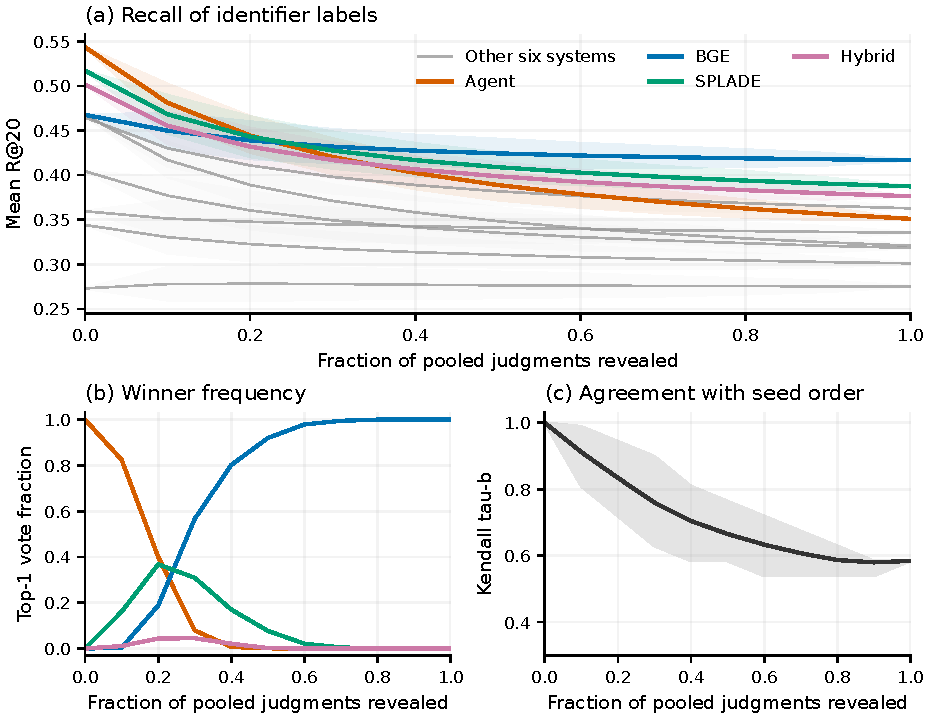
\includegraphics[width=\linewidth]{figures/qrel_disclosure_readable.pdf}
\caption{Controlled nested disclosure of the existing historical judgment pool (1,000 paired replicates; ten systems; 108 fixed supported queries). Panel (a) shows all ten fixed systems, highlighting the four with nonzero observed top-1 votes; six others are gray. Panel (b) shows tie-adjusted top-1 frequencies and (c) tie-aware rank agreement. Bands in (a) and (c) are central empirical disclosure intervals, not population confidence intervals; panel (b) shows point frequencies only. These are conditional identifier-level diagnostics, not biomedical retrieval accuracy. Full disclosure reconstructs 1,370 positive pairs.}
\label{fig:disclosure}
\end{figure}

\subsection{Results and statistical interpretation}
The leader by mean token $\Rtwenty$ across replicates is the agent at $f=0.2$ and BGE at $f=0.3$. This brackets a change on the tested grid between six and nine revealed judgments per query. It is not an estimated continuous crossover threshold, evidence of monotonicity, or a universal judgment-budget prescription.

\begin{table}[t]
\centering
\caption{Paired conditional disclosure results. $\Delta=M_{\mathrm{BGE}}-M_{\mathrm{agent}}$. Intervals are the empirical 2.5th--97.5th percentiles of 1,000 paired differences, not confidence intervals for a population mean. Top-1 votes are split among exact ties across all ten systems.}
\label{tab:disclosure}
\begin{tabular}{@{}rrrrr@{}}
\toprule
$f$ & Revealed/query & Mean $\Delta$ & Empirical 95\% interval & BGE top-1 \\
\midrule
0.2 & 6 & $-0.005432$ & $[-0.030669,\;0.020421]$ & 18.8\% \\
0.3 & 9 & $0.011653$ & $[-0.013106,\;0.035547]$ & 56.7\% \\
0.4 & 12 & $0.024971$ & $[0.001644,\;0.047598]$ & 80.2\% \\
0.5 & 15 & $0.035463$ & $[0.014555,\;0.056464]$ & 92.0\% \\
1.0 & 30 & $0.065735$ & $[0.065735,\;0.065735]$ & 100\% \\
\bottomrule
\end{tabular}
\end{table}

At both $f=0.2$ and $f=0.3$, paired empirical intervals include zero (Table~\ref{tab:disclosure}). BGE strictly exceeds the agent in 34.9\% and 83.1\% of replicates, respectively, but wins against all ten systems in only 18.8\% and 56.7\%. These are distinct statistics: beating one comparator does not imply winning overall. At $f=0.5$, BGE receives 92.0\% of top-1 votes. At full disclosure it receives every vote, deterministically conditional on these fixed inputs. Intermediate observed rates of zero or one in 1,000 replicates do not prove impossibility or certainty under the disclosure distribution.

Kendall's $\tau_b$ complements the leader plot because it measures pairwise order agreement throughout the system list and corrects for ties. The seed ordering ties BM25 and BGE, so a tie-ignorant coefficient would conflate breaking that tie with reversing a strict preference. Average ranks similarly preserve ties; strict reversals require opposite nonzero signs. Spearman correlation provides a rank-displacement summary of the endpoints, not an independent significance test. Definitions are in Appendix~\ref{app:stats}.

The randomness here concerns which already judged records are revealed, conditional on the selected pool, automated verdicts, seeds, queries, and saved rankings. The intervals are not uncertainty about a biomedical population, true relevance, or a model's future performance. Randomly disclosing records from a biased pool does not model missing-not-at-random unknown relevance outside it. Candidate-origin system fields were not retained in the raw judgments, so a provenance-grounded leave-one-system-out pooling analysis cannot be recovered. Ranking overlap is not a substitute for those missing origins.

\section{What the Repaired Infrastructure Establishes}
\label{sec:software}
\subsection{Actual local retrieval, without accuracy claims}
The restored dataset was indexed using a hash-bound inverted BM25 implementation. It contains 4,936 documents, 10,313 chunks, 63,109 lexical vocabulary terms, and 2,010,185 postings. Document selection uses the original query's maximum chunk score, with stable index-order ties. This transparent implementation supports equation checks rather than relying on an unverified legacy serialized index.

Eight predeclared, unscored probes were run under three non-LLM conditions: original-query top-24, repeated original query with three batches of eight new documents, and deterministic token-window reformulation. All 24 local runs completed with 24 unique candidates. For every probe, repeated-original and original-top-24 produced exactly the same candidates and primary selection, as expected for stable ranking with adequate candidates. Independent naive-formula comparisons numbered 290, with maximum absolute error $7.1054\times10^{-15}$. These checks support implementation correctness and integration, not retrieval accuracy or the probes' intended scientific capabilities.

Recorded build and verified-load times were 3.16048 and 2.28054 seconds. Single loaded-index prefix-search measurements over the eight probes ranged from 0.923 to 1.524 milliseconds, with median 1.182 milliseconds. These are bounded local systems measurements, not a latency guarantee; they do not include a live model workflow. Separate native-adapter checks yielded 56 dry condition plans and 24 offline retrieval checks, with zero provider/model calls. These are not additional model experiments.

\subsection{Structural success and selective evaluation contracts}
\label{sec:structural}
Document recall does not measure whether the retrieved set satisfies a comparison, contradiction relation, or multi-hop chain. A tested evaluator therefore accepts explicit evidence units and relations rather than inferring them from seed labels. Let $S$ be the retrieved document prefix, $U$ the required units, and $E(d)\subseteq U$ the units annotated for document $d$. Common diagnostics are
\begin{equation}
 C(S)=\frac{|\bigcup_{d\in S}E(d)|}{|U|},\qquad
 A(S)=\ind\!\left[U\subseteq\bigcup_{d\in S}E(d)\right].
\end{equation}
Family success is more specific. Comparison requires both annotated sides. Contradiction requires some explicitly valid pair $p$ with $p\subseteq S$, and multi-hop requires some annotated valid path $p\subseteq S$; path membership, not retrieval order, determines completion. Joint constraint success requires $\exists d\in S:U\subseteq E(d)$ unless an explicit set-level policy permits union completion. Temporal and aggregation success require all annotated time bins or study-value units, respectively. Negative-result success requires evidence explicitly annotated with the negative finding. Arbitrarily combining halves of different paths must not pass merely because their union covers every unit.

These are implemented contracts tested on software fixtures, not measured structural scores for the historical or restored corpus. Missing annotations yield null metrics and denominator zero, not seed-derived success. Unvalidated annotations can only enter a separately labeled descriptive-proxy mode. The evaluator's status fields cannot authenticate a claimed adjudication; no such real human adjudication was performed here.

Selective evaluation likewise distinguishes \texttt{ANSWER}, \texttt{ABSTAIN}, and \texttt{UNCERTAIN}. Coverage uses all expected tasks; risk requires external evidence-set failure labels for the answered sets. Empty qrels do not establish appropriate abstention, and uncertain decisions are not relabeled as verified corpus absence. Consequently, this paper reports neither scientific answer accuracy nor calibrated selective risk.

\subsection{Candidate budgets do not isolate an iteration mechanism}
Seven implemented protocols share a cap of 24 unique candidate documents and an original-query final selector: three non-LLM controls, one-shot rewrite, upfront three queries, evidence feedback, and feedback without accumulated evidence. Fixture tests and real-corpus dry checks exercise the interfaces; no live LLM condition has been evaluated. The heuristic is token-window reformulation, not RM3 or learned relevance feedback.

Equal candidate count does not imply equal compute, prompt tokens, observed evidence, or cost. In the planned feedback schedules, accumulated feedback would expose eight then sixteen documents, whereas the no-accumulation condition would expose eight then eight; both retain query history. This exposure confound prevents an isolated interpretation of memory or iteration. We therefore withdraw any claim that historical differences establish an ``iteration mechanism.'' A causal comparison would require executed, provenance-bound controls and an explicit choice of which resources and observations are matched.

\section{Discussion and Limitations}
The combined audit separates two mechanisms that should not be conflated. Changing the supplied relevance labels changes system order while saved rankings remain fixed. Correcting source identity changes which scientific text can legitimately be associated with an identifier. The first is measured by conditional token arithmetic; the second is supported by authoritative metadata and own-article XML checks. We have not measured a corrected-corpus ranking change, and do not attribute the observed nine reversals causally to the parser bug.

The case nevertheless reveals an important failure mode for benchmark interpretation. Recomputing a table exactly is insufficient when source identity is wrong; repairing source identity is insufficient when relevance labels are biased or invalid. A valid reconstruction must preserve separate evidence for the two operations. In this study, that separation prevents a tempting but unsupported repair: simply rewriting historical labels onto new canonical IDs and presenting the rescored outputs as a new benchmark.

Several limits remain substantial. The collection is synthetic and historically exposed; no new source-disjoint task partition exists. Seed positives are forced by construction, and the expanded pool contains automated judgments rather than independently adjudicated relevance. Historical generation and judging used a proprietary model, and this audit does not recreate its original service state or establish cross-model robustness. The disclosure design quantifies variation within a finite biased pool, not its completeness. The source snapshot reflects current metadata, so not every discrepancy can be attributed to the old parser. Restoration is partial, with title-only documents and lossy formula/table rendering. Tests validate specified structural behavior, not scientific semantics. Finally, source ownership and retained license statements do not authorize blanket redistribution of article text.

\section{Conclusion}
A joint provenance and label audit changes what can responsibly be concluded from \cer. The authoritative re-fetch identifies cited-identifier contamination, while fixed historical rankings show nine pairwise reversals under alternative label sets. Nested disclosure locates a change of the mean-score leader between tested fractions 0.2 and 0.3, with overlapping-zero paired empirical intervals at both points. The new source-owned retrieval dataset and local BM25 checks establish a reproducible substrate, not a corrected biomedical leaderboard. The defensible outcome is an audited boundary between reproducible arithmetic, verified source identity, and still-unvalidated relevance.
\label{page:mainend}

\section*{Reproducibility Statement}
The retained artifacts include raw PubMed request logs and XML hashes, all-record comparisons, source-owned text manifests and offsets, exact historical token arithmetic, disclosure permutations and score arrays, and local retrieval traces. The disclosure experiment fixes its random generator, seeds, query universe, and tie policy; all endpoint means match exact rational references. The manuscript's companion claim ledger maps claims to repository-relative evidence. No new model calls are required to reproduce the disclosed token calculations or local source/index checks. Provider-dependent historical generation is not independently reproduced. The final integrated software suite passes all 311 tests with no failures or skips; this establishes software verification, not independent biomedical validation.

\section*{Ethics and AI-Use Statement}
This work analyzes published scientific-source records and synthetic tasks; it reports no participant study or human relevance-annotation study. Human validation was not performed. AI assistance was used for code development, audit analysis, and manuscript preparation; this does not constitute independent relevance assessment. Historical task generation and judging relied on a proprietary language model. Neither those judgments nor this audit should be used as clinical advice or evidence of biomedical correctness. Retained provenance supports local research inspection; it does not establish that all article text may be redistributed. No public-release or blanket licensing approval is claimed.

\bibliography{refs}
\bibliographystyle{iclr2027_conference}

\appendix
\section{Statistical Definitions and Scope}
\label{app:stats}
\paragraph{Fixed universe and exact means.}
The historical test universe contains 125 rows per system. Metrics condition on the same 108 tasks with nonempty seed labels at all disclosure fractions. Since seeds are retained, their denominators never become zero. The remaining 17 rows have null retrieval metrics and remain explicitly excluded, not dropped from coverage accounting. Each supported query has equal weight $1/108$, regardless of its positive-label count. Exact common-denominator integer arithmetic determines ordering before conversion to floating-point display values.

\paragraph{Pairing and empirical intervals.}
For a pair of methods $a,b$, let $D_r(f)=M_{a,r}(f)-M_{b,r}(f)$. Reported differences average these 1,000 paired values; interval endpoints are their empirical 0.025 and 0.975 quantiles. They describe how scores vary when a fixed finite pool is partially disclosed. They are not bootstrap confidence intervals, hypothesis tests, or confidence bounds on a win probability. Queries and their underlying judgments are not resampled. At $f=0$ and $f=1$, label sets are fixed across replicates, so their conditional intervals collapse to points by design.

\paragraph{Top-1 votes and strict exceedance.}
Let $W_r(f)$ be the set of methods attaining the exact largest mean in replicate $r$. Method $s$ receives vote $v_{s,r}(f)=\ind[s\in W_r(f)]/|W_r(f)|$. Its top-1 rate is $1000^{-1}\sum_r v_{s,r}(f)$; votes sum to one per replicate. Pairwise strict exceedance instead averages $\ind[D_r(f)>0]$. Neither quantity is the probability that a method is best for biomedical users. The manuscript reports rates, not per-replicate vote quantiles as if they were confidence bounds on those rates.

\paragraph{Strict reversals.}
For systems $a,b$, a reversal relative to the seed regime occurs if
\begin{equation}
 (M_a(0)-M_b(0))(M_{a,r}(f)-M_{b,r}(f))<0.
\end{equation}
A broken seed tie is not a reversal. There are $\binom{10}{2}=45$ possible pairs, including the seed-tied pair in the reporting denominator. Thus nine endpoint reversals correspond to $9/45$, not a denominator that silently excludes inconvenient pairs.

\paragraph{Rank correlations.}
For two score vectors over the same ten methods, let $C,D$ count concordant and discordant pairs, and $T_x,T_y$ count pairs tied only in the first or second vector. Kendall's coefficient is
\begin{equation}
 \tau_b=\frac{C-D}{\sqrt{(C+D+T_x)(C+D+T_y)}}.
\end{equation}
Average ranks are assigned to exact ties. Spearman's $\rho$ is the Pearson correlation of these rank vectors. The saved disclosure implementation computes tie-aware agreement between fraction pairs; 363 comparisons against an independent SciPy calculation were recorded. The correlations summarize conditional system order, not relevance validity.

\paragraph{Why no cross-regime recall-drop interpretation?}
Writing $G'=G\cup H$ changes recall to $(|T\cap G|+|T\cap(H\setminus G)|)/(|G|+|H\setminus G|)$. A fixed ranking may score lower even while retrieving additional newly labeled positives, because the denominator grows faster. Consequently, numerical endpoint differences across seed and expanded regimes are not performance deterioration from a model intervention. Within-fraction paired differences compare systems under the same label sets; across-fraction order changes diagnose dependence on those sets.

\section{Direct-Child Identity Extraction and Audit Root Cause}
\label{app:parser}
The essential ownership rule is to select identifiers from the current article's own metadata container. The following pseudocode omits transport and normalization details but makes the traversal boundary explicit:
\begin{verbatim}
for record in returned_pubmed_records:
    citation = direct_child(record, "MedlineCitation")
    pmid = required_unique_text(direct_child(citation, "PMID"))
    pubmed_data = direct_child(record, "PubmedData")
    own_list = direct_child(pubmed_data, "ArticleIdList")
    own_ids = direct_children(own_list, "ArticleId")
    pmc = unique_or_absent(own_ids, type="pmc")
    doi = unique_or_absent(own_ids, type="doi")
    if doi is absent:
        article = direct_child(citation, "Article")
        doi = own_elocation_doi_or_absent(article)
    emit(pmid, normalize_pmc(pmc), doi)
    # Never fill absent own IDs from ReferenceList descendants.
\end{verbatim}
Actual parsing supports namespace-qualified elements and rejects conflicting identities. Repeated identical IDs within one own list are allowed; duplicate returned article records are not. The title and abstract extraction preserves mixed-inline text with \texttt{itertext()}, within explicitly selected own fields. Publication-type and other metadata differences may reflect both updated source content and parser policy, which is why Table~\ref{tab:identity} does not equate every changed row with bug contamination.

The 26 retained batch downloads contain all intended PMIDs after recovery. Two requests each omitted one intended PMID, and another requested an invalid identifier instead of the intended PMID. A supplemental batch recovered the three intended records. This yielded 4,937 unique requested IDs including one invalid non-corpus ID, but 4,936 returned unique corpus PMIDs. An absent optional field in a valid returned record is not a missing article: the snapshot has 2,295 records without PMC identifiers, 20 without DOI, and 22 without abstracts.

The full-text boundary is analogous: use own \texttt{front/article-meta/article-id}, not filename inference, arbitrary body IDs, or reference IDs. A single-article wrapper may be deterministically unwrapped; ambiguous multi-article structures are rejected. Major local-title mismatches quarantine local bodies without invalidating the separate authoritative PubMed metadata. These rules avoid turning a valid metadata record into an unverified full-text association.

\section{Trace, Schema, and Data Availability}
\label{app:trace}
\paragraph{Historical evidence.}
Raw pooled records contain \texttt{task\_id}, \texttt{doc\_id}, and \texttt{judgment}; they do not preserve a candidate-origin system field. The forensic report preserves stored and reconstructed qrels separately, including the exact missing-pair effect. The disclosure artifact retains query/candidate order, all per-query permutations, random seeds, exact score units and divisor, floating means, average ranks, top-1 votes, reversal arrays, and tie-aware rank agreements. Its manifest binds the inputs, code, configuration, and outputs. No corpus record is dereferenced in that disclosure experiment.

\paragraph{New retrieval data.}
Each document and chunk carries a canonical \texttt{doc\_id}, matching \texttt{article\_id}, and a common versioned \texttt{corpus\_id}. Each chunk has a unique opaque \texttt{chunk\_id} and explicit text. Offsets are half-open Unicode-codepoint offsets in rendered text, not byte positions in raw XML. Source blocks retain source type, XML locator, raw path/hash, section ownership, and intersections with chunk-relative and document-relative ranges. Explicit rendering additions include block separators and table-cell coordinate labels. Retained nonindexed local abstracts are distinguished from indexed authoritative abstracts to avoid duplicate indexing.

\paragraph{Protocol traces.}
The implemented budget protocol distinguishes logical searches, cache hits, ranked chunk output, admitted candidates, and model-visible observations. A full retrieval ranking is not automatically a model observation. Candidate admission is document-deduplicated; each admitted document supplies a representative chunk. The intended model trace includes request, response, displayed evidence, usage when available, latency, and typed errors. Character clipping is not token accounting. Dry plans contain no actual API observations or model responses, and cannot be resumed as completed experiments.

\paragraph{Availability and rights.}
The accompanying repository materials are identified by relative paths in \path{CLAIMS_TO_ARTIFACTS.md}. Principal locations are \path{results/readiness/authoritative_corpus/}, \path{results/readiness/verified_fulltext/}, \path{results/readiness/qrel_sensitivity/v1_forensic/}, and \path{results/readiness/qrel_disclosure/v2/}. The new dataset resides under \path{data/processed/authoritative_fulltext_v1/}. These locations describe retained artifacts, not a claim of an already completed public release. Public PubMed endpoints identify the metadata sources; local article text remains subject to source-specific permissions. License recognition is not license adjudication, and public redistribution has not been authorized by this audit.

\section{Software Verification Versus Scientific Evidence}
The authoritative-parser evidence records 51 targeted/adjacent passing tests at its snapshot. The restoration evidence records 83 passing tests and byte-identical independent builds. The disclosure evidence records 11 passing tests and exact agreement of 20 rational endpoints. The real-corpus retrieval evidence records 68 passing tests and 290 independent formula comparisons. These suites overlap; their counts must not be summed into a count of unique tests or independent scientific replications.

An intermediate adapter verification encountered a stale historical source-hash assertion; its failed and filtered-run receipts are preserved. A subsequent, separately versioned native-backend integration retained strict provenance checks, reused the immutable index, and bound the updated sources. The final complete configured suite passes 311 tests with no failures, errors, skips, or deselection. Twenty-four actual offline retrieval checks and 24 separate dry plans ran in that integration, with zero model calls. Old build timings and formula comparisons are explicitly identified as historical measurements rather than presented as rerun measurements. Snapshot-specific checks remain important because a legitimate source change can invalidate an earlier attestation.

Neither these tests nor programmatically fictional structural fixtures are human experiments. Simulated adjudication statuses in fixtures test software branches; they must not be interpreted as annotations for real papers. Future scientific evaluation would need new tasks tied to the corrected source version, independently justified evidence relations, and explicit split/exposure control. Any future automated-only results would still require the absence of human validation to remain visible. The present manuscript does not fill this gap with historical gold migration, fabricated structural scores, or unexecuted model comparisons.
\end{document}
